\documentclass[uplatex]{jsarticle}

\usepackage[dvipdfmx]{graphicx}
\usepackage[dvipdfmx]{color}
\usepackage{caption}
\usepackage{float}
\usepackage{amsmath}

\setlength{\textheight}{244truemm}
\setlength{\headheight}{0pt}
\setlength{\headsep}{25truemm}
\setlength{\footskip}{15truemm}
\addtolength{\topmargin}{-1truein}

\title{電子制御工学実験II課題レポート}
\author{EC2 37番 平田蓮}
\date{2018/7/18}

\begin{document}
    \begin{figure}[h]
        \begin{center}
            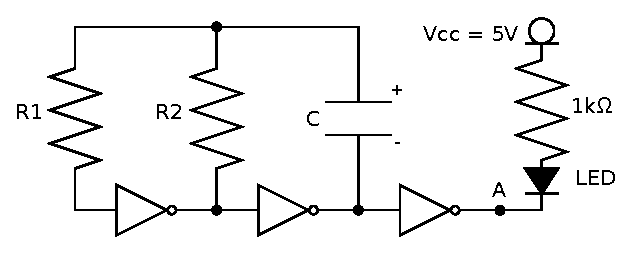
\includegraphics{1.eps}
            \caption{NOTを使ったRC発振回路}
            \label{NOTを使ったRC発振回路}
        \end{center}
    \end{figure}
    \subsubsection*{課題1}
        図\ref{NOTを使ったRC発振回路}の発振回路の動作原理を図を示しながら解説せよ.\par
        \begin{figure}[h]
            \begin{center}
                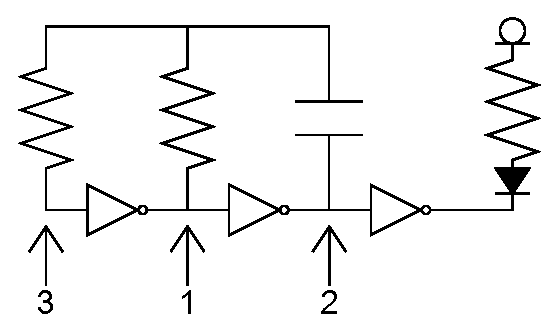
\includegraphics{2.eps}
                \caption{RC発振回路}
                \label{RC発振回路}
            \end{center}
        \end{figure}
        図\ref{RC発振回路}の1番の部分の電圧が高まると,2,3に電流が流れこみ次第にコンデンサに充電されていき,一定の値を超えると,放電が始まる.すると,逆に1の部分に電流が流れ込む.
        この繰り返しの中で,A地点での入力,出力が切り替わる.
    \newpage
    \subsubsection*{課題2}
        発振回路の出力波形はどうなるか,図を描き説明せよ.\par
        \begin{figure}[h]
            \begin{center}
                \includegraphics{3.eps}
                \caption{発振回路の波形}
                \label{発振回路の波形}
            \end{center}
        \end{figure}
        図\ref{発振回路の波形}のように,急に,ハイ出力とロー出力が切り替わる波形になる.これは,一定の電圧によってハイとローを切り替えているためである.
    \begin{table}[h]
        \caption{抵抗と静電容量の組み合わせによる周波数の変化}
        \label{抵抗と静電容量の組み合わせによる周波数の変化}
        \begin{center}
            \begin{tabular}{c|c|c|c|c|c}\hline
                抵抗値 & \multicolumn{5}{|c}{コンデンサ 静電容量 $C [\mathrm \mu F]$} \\ \cline{2-6}
                $R1,R2[k \mathrm \Omega]$ & 0.1 & 1.0 & 2.2 & 4.7 & 10 \\ \hline
                1.0 & $4.0 \times 10^{3}$ & $5.0 \times 10^{2}$ & $2.2 \times 10^{2}$ & $1.0 \times 10^{2}$ & 45 \\ \hline
                2.0 & $2.0 \times 10^{3}$ & $2.5 \times 10^{2}$ & $1.1 \times 10^{2}$ & 50 & 23 \\ \hline
                3.0 & $1.3 \times 10^{3}$ & $1.7 \times 10^{2}$ & 72 & 32 & 15 \\ \hline
                4.3 & $9.3 \times 10^{2}$ & $1.2 \times 10^{2}$ & 51 & 23 & 10 \\ \hline
                5.1 & $8.4 \times 10^{2}$ & $1.0 \times 10^{2}$ & 42 & 20 & 9.0 \\ \hline
                6.2 & $7.4 \times 10^{2}$ & 82 & 35 & 16 & 7.3 \\ \hline
                7.5 & $5.7 \times 10^{2}$ & 68 & 29 & 13 & 6.0 \\ \hline
                8.2 & $5.4 \times 10^{2}$ & 63 & 26 & 12 & 5.5 \\ \hline
                9.1 & $5.2 \times 10^{2}$ & 56 & 24 & 12 & 4.9 \\ \hline
                10.0 & $4.3 \times 10^{2}$ & 51 & 21 & 9.5 & 5.0 \\ \hline
            \end{tabular}
        \end{center}
    \end{table}
    \subsubsection*{課題3}
        抵抗値を変化させると,出力波形の周波数はどのように変化するか.\par
        表\ref{抵抗と静電容量の組み合わせによる周波数の変化}より,抵抗が増えれば増えるほど,周波数は低下する.
    \subsubsection*{課題4}
        コンデンサの静電容量を変化させると,出力波形の周波数はどのように変化するか.\par
        表\ref{抵抗と静電容量の組み合わせによる周波数の変化}より,静電容量が増えれば増えるほど,周波数は低下する.
    \subsubsection*{課題5}
        表\ref{抵抗と静電容量の組み合わせによる周波数の変化}より,抵抗値と静電容量から周波数を求めるための式を導け.\par
        周波数を見てみると,抵抗値,静電容量のどちらにも反比例していることがわかる.よって,周波数は,
        \begin{flalign*}
            \frac{x}{RC} \quad (xは定数)
        \end{flalign*}
        の形で表せる.
        表の値を代入して,定数$x$の平均値を求めると,$0.47$になる.よって,
        \begin{flalign*}
            \frac{0.47}{RC}
        \end{flalign*}
        この式で周波数を求めることができる.
\end{document}
